% Latex template: mahmoud.s.fahmy@students.kasralainy.edu.eg
% For more details: https://www.sharelatex.com/learn/Beamer

\documentclass[1610]{beamer}					  % Document class

\usepackage[portuguese]{babel}			  % Set language
\usepackage[utf8x]{inputenc}			  % Set encoding

\mode<presentation> {					  % Set options
  \usetheme{default}					    % Set theme
  \usecolortheme{default} 				% Set colors
  \usefonttheme{default}  				% Set font theme
  \setbeamertemplate{caption}[numbered]	% Set caption to be numbered
}

\setbeamertemplate{navigation symbols}{}
\setbeamertemplate{footline}[frame number]
\setbeamercovered{transparent}

\newcommand\Wider[2][3em]{%
\makebox[\linewidth][c]{%
  \begin{minipage}{\dimexpr\textwidth+#1\relax}
  \raggedright#2
  \end{minipage}%
  }%
}

% Uncomment this to have the outline at the beginning of each section highlighted.
%\AtBeginSection[]
%{
%  \begin{frame}{Outline}
%    \tableofcontents[currentsection]
%  \end{frame}
%}

\usepackage{graphicx}					% For including figures
\usepackage{booktabs}					% For table rules
\usepackage{hyperref}					% For cross-referencing
\usepackage{caption}                    % Allows more control over captions in figs and tables

\title{Revisão de Atividades da FAC}	% Presentation title
%\author{Author One}					% Presentation author
\institute{LNLS.DAC.FAC}				% Author affiliation
\date{2024-03-08 -- 2024-04-19}			% Today's date	


\begin{document}



\begin{frame}
  \titlepage
  \href{https://github.com/lnls-fac/doc-review-dac-fac}{\beamergotobutton{Link para o repo github desta apresentação: https://github.com/lnls-fac/doc-review-dac-fac}}
  \href{https://www.overleaf.com/read/sbdjxtzfchrm}{\beamergotobutton{Link para o projeto overleaf destas notas}}
\end{frame}

\begin{frame}{Outline}
  \tableofcontents
\end{frame}

% Machine studies in the period

% 2024-03-11-FOFB-Acq
% 2024-03-12-SI_llrf_study
% 2024-03-19-SI_NLK
% 2024-03-19-SI_bpms_equalization
% 2024-03-22-SI_hla_problem
% 2024-03-25-SI_FOFB_Study
% 2024-03-25-SI_FOFB_respmat_alternatives
% 2024-03-25-SI_llrf_study
% 2024-03-25-SI_tune-tracking-sigmay-control
% 2024-04-01-BO_beam_images_at_screens
% 2024-04-01-SI_injection_collimation_with_scrapers
% 2024-04-01-SI_orbit_stability_hydraulic_valve_10hz_problem
% 2024-04-12-coldbox-orbit-acqs
% 2024-04-16-SI-delta-optics-ffwd
% 2024-04-16-SI_NLK
% 2024-04-16-SI_boramp_effect_orbit_acq

\section{Estudos com LLRF}

\begin{frame}
    \Huge{Estudos com LLRF}
\end{frame}

\begin{frame}{Estudos de máquina}
\begin{itemize}
    \item 2024-03-12 $\to$ explorar parâmetros de controle, medidas para paper IPAC, crosstalk entre FOFB e LLRF observado
    \item 2024-03-25 $\to$ explorar crosstalk entre FOFB e LLRF
\end{itemize}
\end{frame}

\begin{frame}{}
\centering
\Wider[4em]{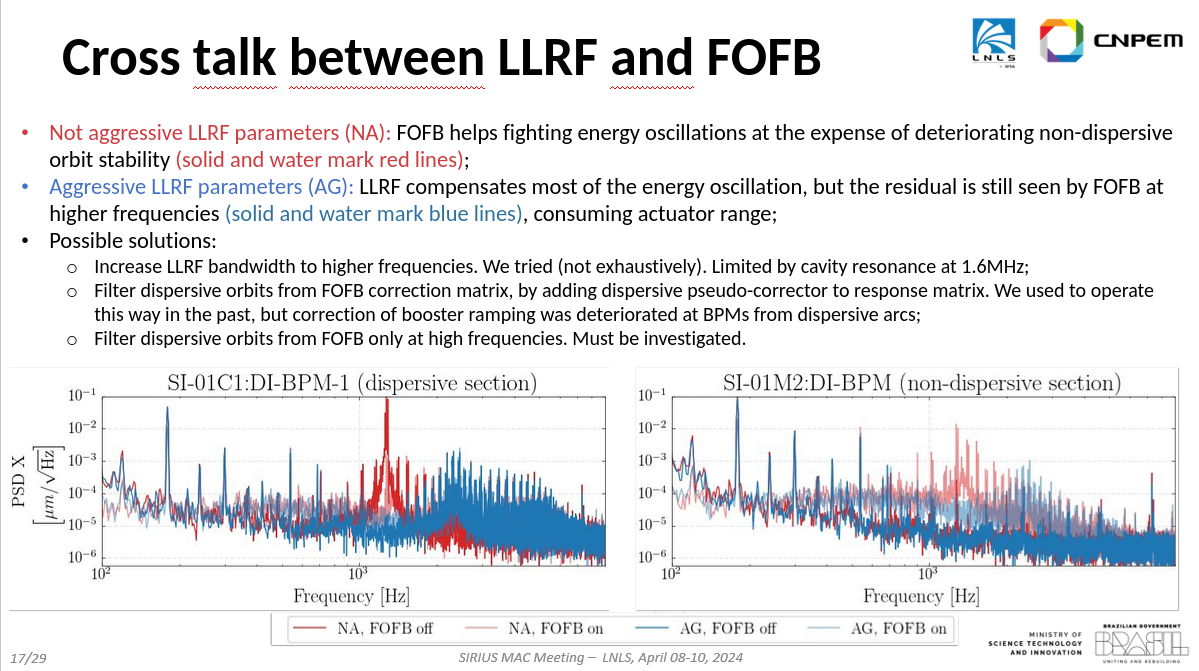
\includegraphics[scale=0.29]{2024-04-19/figures/crosstalk_llrf_fofb.png}}
\end{frame}

\section{Testes de controle de emitância com bunch-by-bunch}

\begin{frame}
    \Huge{Testes de controle de emitância com bunch-by-bunch}
\end{frame}

\section{Testes de colimação de injeção com scrapers}

\begin{frame}
    \Huge{Testes de colimação de injeção com scrapers}
\end{frame}

\section{Estabilidade de órbita}

\begin{frame}
    \Huge{Estabilidade de órbita}
\end{frame}

\begin{frame}{O mistério em 10Hz}
    
\end{frame}

\section{MAC Meeting}

\begin{frame}
    \Huge{MAC Meeting}
\end{frame}

\begin{frame}{Apresentações FAC}
Entre 08 de Março
    \begin{itemize}
        \item 03 - Beam Stability
        \item 08 - Progress on Third Harmonic Cavities Studies
        \item 13 - Injection System
        \item 14 - Nonlinear Dynamics
    \end{itemize}
\end{frame}


\end{document}
